\section{Minimum Spanning Trees}\label{sec:2}

\subsection{Trees}\label{subsec:2.1}
A {\bf tree} is a connected acyclic graph; that is, a connected graph 
containing no cycles. 
\begin{center}
    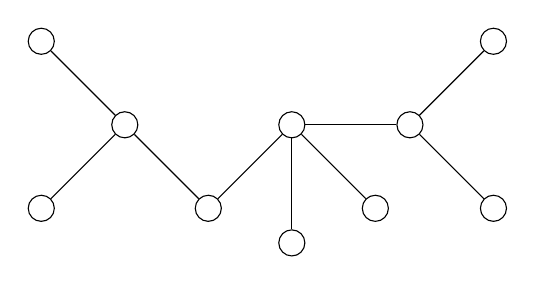
\begin{tikzpicture}[node distance={15mm}, main/.style = {draw, circle}] 
        \node[main] (1) {}; 
        \node[main] (2) [below right of=1] {};
        \node[main] (3) [below left of=2] {}; 
        \node[main] (4) [below right of=2] {};
        \node[main] (5) [above right of=4] {};
        \node[main] (6) [below of=5] {};
        \node[main] (7) [below right of=5] {};
        \node[main] (8) [right of=5] {};
        \node[main] (9) [above right of=8] {};
        \node[main] (10) [below right of=8] {};

        \draw (1) -- (2); \draw (2) -- (3); \draw (2) -- (4);
        \draw (4) -- (5); \draw (5) -- (6); \draw (5) -- (7);
        \draw (5) -- (8); \draw (8) -- (9); \draw (8) -- (10);
    \end{tikzpicture} 
\end{center}
\vspace{-0.25cm}
Given a graph $G = (V, E)$, a {\bf spanning tree} of $G$ is a graph $T = (V, F)$ 
such that $F \subseteq E$ and $T$ is a tree. We illustrate an example of a 
graph $G$ with a subtree $T$ using bold edges below. 
\begin{center}
    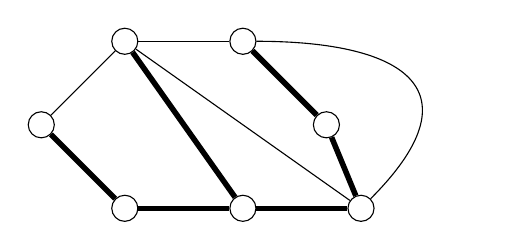
\begin{tikzpicture}[node distance={15mm}, main/.style = {draw, circle}] 
        \node[main] (1) {}; 
        \node[main] (2) [right of=1] {};
        \node[main] (3) [below left of=1] {}; 
        \node[main] (4) [below right of=2] {};
        \node[main] (5) [below right of=3] {};
        \node[main] (6) [right of=5] {};
        \node[main] (7) [right of=6] {};

        \draw (1) -- (2); 
        \draw (1) -- (3); 
        \draw [line width=2pt] (1) -- (6);
        \draw (1) -- (7);
        \draw [line width=2pt] (2) -- (4);
        \draw (2) to [out=0, in=45, looseness=2] (7);
        \draw [line width=2pt] (3) -- (5);
        \draw [line width=2pt] (4) -- (7);
        \draw [line width=2pt] (5) -- (6);
        \draw [line width=2pt] (6) -- (7);
    \end{tikzpicture} 
\end{center}
In an introductory graph theory course, such as MATH 239, 
it is shown that every tree on $n$ vertices has $n-1$ edges. The following 
theorem then gives us a useful characterization of trees. 

\begin{theo}[Fundamental Theorem of Trees]{theo:2.1}
    Let $T = (V, F)$ be a graph. The following are equivalent:
    \begin{enumerate}[(i)]
        \item $T$ is a tree. 
        \item $T$ is connected and $|F| = |V| - 1$. 
        \item $T$ is acyclic and $|F| = |V| - 1$. 
    \end{enumerate}
\end{theo}\vspace{-0.25cm}

In particular, if we know that two of the conditions hold, then the 
third one is guaranteed.

\subsection{Minimum Spanning Trees}\label{subsec:2.2}
Given a connected graph $G = (V, E)$ and edge costs $c_e$ for each 
$e \in E$, our goal is to find a spanning tree $T$ of minimum cost 
\[ c(T) := \sum_{e \in T} c_e. \] 
First, we'll set some notation. For a vertex $v \in V$, we define 
$\delta(v)$ to be the set of edges in $E$ incident to $v$. More generally, 
given a subset of vertices $S \subseteq V$, the {\bf cut induced by $S$} is 
defined to be the set 
\[ \delta(S) := \{uv \in E : u \in S,\, v \notin S\}. \] 
The following theorem will be extremely important for finding a minimum 
spanning tree. 

\begin{theo}[Cut Property]{theo:2.2}
    Suppose that the costs $c_e$ for $e \in E$ are distinct. 
    Let $S \subseteq V$ be such that $S \neq \varnothing$ and $S \neq V$, 
    and let 
    \[ e = \argmin_{f \in \delta(S)} c_f. \] 
    Then every minimum spanning tree contains the edge $e$. 
\end{theo}\vspace{-0.25cm}
\begin{pf}[Theorem~\ref{theo:2.2}]
    We proceed by contradiction. Let $S \subseteq V$ be such that $S 
    \neq \varnothing$ and $S \neq V$, and let $e = \argmin_{f\in S} c_f$. 
    Suppose that there is a minimum spanning tree $T = (V, F)$ such that 
    $e \notin F$. 

    Consider the graph $(V, F \cup \{e\})$. Note that $|F \cup \{e\}| = |V|$ 
    and this graph is connected, so it cannot be a tree by Theorem~\ref{theo:2.1}. 
    In particular, it must contain a cycle $C$. 

    Next, note that $|C \cap \delta(S)|$ must be even because for any 
    edge leaving the cut $\delta(S)$, there must be another edge coming back 
    into the cut. Moreover, since $e \in C \cap \delta(S)$, we have 
    $C \cap \delta(S) \neq \varnothing$. This implies that 
    $|C \cap \delta(S)| \geq 2$, so there is another edge $e' \neq e$ 
    with $e' \in C \cap \delta(S)$.

    Consider now the graph $T' = (V, (F \cup \{e\}) \setminus \{e'\})$. 
    Then $|(F \cup \{e\}) \setminus \{e'\}| = |F| = |V| - 1$ and $T'$ is 
    connected because if a path between two vertices used the edge $e'$, 
    then we could go along the edges in $C \setminus \{e'\}$ instead. 
    So by Theorem~\ref{theo:2.1}, $T'$ is also a spanning tree. 
    Finally, observe that 
    \[ c(T) - c(T') = c_{e'} - c_e > 0 \] 
    because we have $e = \argmin_{f\in S} c_f$ and $e' \neq e$ with 
    $e' \in \delta(S)$, as well as the assumption that the edge 
    costs $c_e$ for $e \in E$ were distinct. But $T'$ has lower cost 
    than $T$, contradicting our assumption that $T$ was a minimum 
    spanning tree. \qed
\end{pf}\vspace{-0.25cm}

The following property relating cycles to minimum spanning trees 
can also be proved similarly to Theorem~\ref{theo:2.2}. 
The main idea is to try to create shortcuts using the edges in the cycle. 

\begin{theo}[Cycle Property]{theo:2.3}
    Let $G = (V, E)$ be connected with distinct edge costs 
    $c_e$ for $e \in E$. Let $C$ be a cycle in $G$ and let 
    \[ e = \argmax_{f\in C} c_f. \] 
    Then no minimum spanning tree contains the edge $e$. 
\end{theo}

\subsection{Prim's Algorithm}\label{subsec:2.3}
Prim's algorithm takes the idea of the cut property (Theorem~\ref{theo:2.2}) 
and uses it to compute a minimum spanning tree starting from an arbitrary 
vertex $s \in V$. At each iteration of the algorithm, we will keep track of a 
set of a partial tree construction $T$ and vertices $A \subseteq V$ that are 
connected to $s$ in $T$. We finish once we have reached all the vertices in $G$.

\begin{mdframed}[
    linewidth=1pt,
    linecolor=black,
    bottomline=false,topline=false,rightline=false,
    innerrightmargin=0pt,innertopmargin=0pt,innerbottommargin=0pt,
    innerleftmargin=1em,% Distance between vertical rule & proof content
    skipabove=0.75\baselineskip
]
{\bf Input.} A connected graph $G = (V, E)$ and edge costs $c_e$ for 
all $e \in E$. 

{\bf Output.} The edges $T$ of a minimum spanning tree of $G$.
\begin{enumerate}[leftmargin=1.75cm, label={Step \arabic*.}]
    \item {\bf (Initialization.)} Let $s \in V$ be an arbitrary vertex, 
    then set $A \gets \{s\}$ and $T \gets \varnothing$.

    \item While $A \neq V$:
    \begin{enumerate}[label={Step 2.\arabic*.}]
        \item {\bf (Pick an edge for the minimum spanning tree.)} 
        Set 
        \[ e \gets \argmin_{f \in \delta(A)} c_f, \] 
        where $e = uv$ with $u \in A$ and $v \notin A$.  
        \item {\bf (Update values.)} Set $A \gets A \cup \{v\}$ and 
        $T \gets T \cup \{e\}$. 
    \end{enumerate}
\end{enumerate}
\end{mdframed}\vspace{-0.15cm}

Let's run Prim's algorithm on a simple example. Consider the following 
graph $G = (V, E)$, and suppose that at Step 1, we pick $v_1$ to be 
the initial vertex. 
\begin{center}
    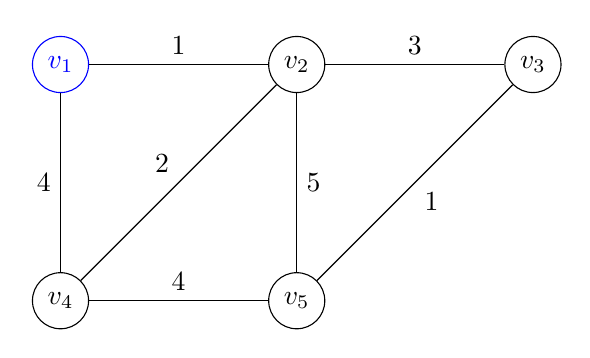
\begin{tikzpicture}[node distance={30mm}, main/.style = {draw, circle}] 
        \node[main, color=blue] (1) {$v_1$}; 
        \node[main] (2) [right of=1] {$v_2$};
        \node[main] (3) [right of=2] {$v_3$}; 
        \node[main] (4) [below of=1] {$v_4$};
        \node[main] (5) [right of=4] {$v_5$};

        \draw (1) -- node[midway, above] {1} (2);
        \draw (2) -- node[midway, above] {3} (3);
        \draw (1) -- node[midway, left] {4} (4);
        \draw (2) -- node[midway, above left] {2} (4);
        \draw (2) -- node[midway, right] {5} (5);
        \draw (3) -- node[midway, below right] {1} (5);
        \draw (5) -- node[midway, above] {4} (4);
    \end{tikzpicture} 
\end{center}
\vspace{-0.25cm}
Then at the first iteration of Step 2.1, we have $\delta(A) = 
\{v_1v_2, v_1v_4\}$, so we pick $e = v_1v_2$ because it has minimum cost.
At Step 2.2, we set $A = \{v_1, v_2\}$ and $T = \{v_1v_2\}$. 

\begin{center}
    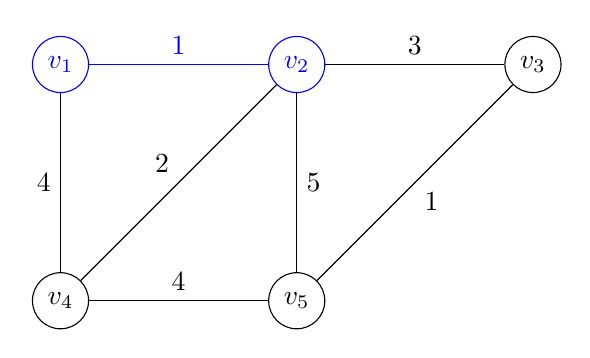
\begin{tikzpicture}[node distance={30mm}, main/.style = {draw, circle}] 
        \node[main, color=blue] (1) {$v_1$}; 
        \node[main, color=blue] (2) [right of=1] {$v_2$};
        \node[main] (3) [right of=2] {$v_3$}; 
        \node[main] (4) [below of=1] {$v_4$};
        \node[main] (5) [right of=4] {$v_5$};

        \draw[color=blue] (1) -- node[midway, above] {1} (2);
        \draw (2) -- node[midway, above] {3} (3);
        \draw (1) -- node[midway, left] {4} (4);
        \draw (2) -- node[midway, above left] {2} (4);
        \draw (2) -- node[midway, right] {5} (5);
        \draw (3) -- node[midway, below right] {1} (5);
        \draw (5) -- node[midway, above] {4} (4);
    \end{tikzpicture} 
\end{center}
\vspace{-0.25cm}
The edge $v_2v_4$ is of minimum cost in the cut induced by $A$, so 
we set $A = \{v_1, v_2, v_4\}$ and $T = \{v_1v_2, v_2v_4\}$ at the next iteration. 
Continuing in this fashion, we obtain the following minimum spanning tree.

\begin{center}
    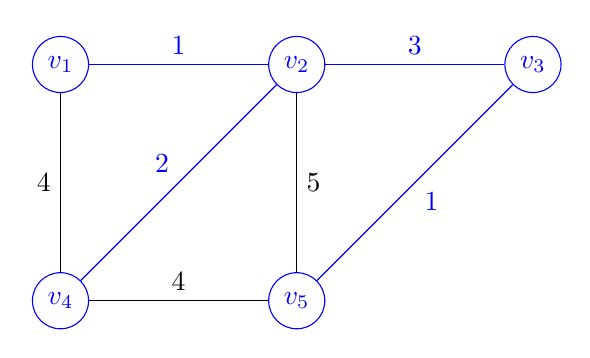
\begin{tikzpicture}[node distance={30mm}, main/.style = {draw, circle}] 
        \node[main, color=blue] (1) {$v_1$}; 
        \node[main, color=blue] (2) [right of=1] {$v_2$};
        \node[main, color=blue] (3) [right of=2] {$v_3$}; 
        \node[main, color=blue] (4) [below of=1] {$v_4$};
        \node[main, color=blue] (5) [right of=4] {$v_5$};

        \draw[color=blue] (1) -- node[midway, above] {1} (2);
        \draw[color=blue] (2) -- node[midway, above] {3} (3);
        \draw (1) -- node[midway, left] {4} (4);
        \draw[color=blue] (2) -- node[midway, above left] {2} (4);
        \draw (2) -- node[midway, right] {5} (5);
        \draw[color=blue] (3) -- node[midway, below right] {1} (5);
        \draw (5) -- node[midway, above] {4} (4);
    \end{tikzpicture} 
\end{center}
\vspace{-0.25cm}
Note that Prim's algorithm may seen similar to Dijkstra's algorithm 
which also yields a spanning tree in the process of computing shortest paths. 
However, these algorithms fundamentally solve different problems, and 
there are examples where the resulting spanning trees do not coincide. 
Moreover, Dijkstra's algorithm takes a directed graph as input, 
whereas Prim's algorithm takes an undirected graph. 

Next, let's prove that Prim's algorithm always gives us a minimum spanning tree. 
For simplicity, we will assume that all edge costs $c_e$ for 
$e \in E$ are distinct. 

\begin{pf}[correctness of Prim's algorithm]
    At every iteration of Step 2, we add one edge to $T$, and we run 
    through $|V| - 1$ iterations. Therefore, $T$ has exactly 
    $|V| - 1$ edges. Moreover, an invariant of Prim's algorithm is that 
    all vertices in $A$ remain connected to $s$, so the final output is 
    also connected. Therefore, we indeed obtain a spanning tree by 
    Theorem~\ref{theo:2.1}. Finally, by the cut property (Theorem~\ref{theo:2.2})
    and our assumption that all the edge costs are distinct, $T$ contains 
    only the edges that are in every minimum spanning tree, so $T$ 
    itself is a minimum spanning tree. \qed 
\end{pf}\vspace{-0.25cm}

As a consequence, we also have the following useful result. 

\begin{cor}{cor:2.4}
    Let $G = (V, E)$ be a connected graph with distinct edge costs $c_e$ for 
    $e \in E$. Then $G$ has a unique minimum spanning tree.
\end{cor}\vspace{-0.25cm}

As usual, let's consider the running time, denoting $|V| = n$ 
and $|E| = m$. For an efficient implementation, 
we keep track of a key $d'(v)$ for each $v \in V \setminus A$. 
Once a vertex $w$ is added to $A$ in Step 2.2, we update the keys via 
$d'(v) \gets \min\{d'(v), c_{wv}\}$ for each $v \in V \setminus A$. 

Note that Step 1 takes $O(1)$ time, and 
there are $n-1$ iterations of Step 2. Implementing Prim's algorithm 
using priority queues, we note that each iteration of Step 2.1 
involves one \textsc{Extract-Min} call, and 
going through all iterations of Step 2.2 takes at most $m$ 
\textsc{Decrease-Key} calls in total. We recall that by using Fibonacci heaps, 
\textsc{Decrease-Key} is $O(1)$ and \textsc{Extract-Min} is $O(\log n)$, 
so we have a total running time of $O(n\log n + m)$.

\subsection{Kruskal's Algorithm}\label{subsec:2.4}
Kruskal's algorithm is another greedy algorithm that finds a minimum 
spanning tree. It first sorts the edges by ascending edge costs 
and continually adds an edge to a partial tree construction $T$ as long as no 
cycle is induced by that edge. The algorithm we give stops once we 
go through every edge, but note that it is enough to stop once the 
number of edges we've added hits $|V| - 1$.

\begin{mdframed}[
    linewidth=1pt,
    linecolor=black,
    bottomline=false,topline=false,rightline=false,
    innerrightmargin=0pt,innertopmargin=0pt,innerbottommargin=0pt,
    innerleftmargin=1em,% Distance between vertical rule & proof content
    skipabove=0.75\baselineskip
]
{\bf Input.} A connected graph $G = (V, E)$ and edge costs $c_e$ for 
all $e \in E$. (We write $m = |E|$ and $n = |V|$.)

{\bf Output.} The edges $T$ of a minimum spanning tree of $G$.
\begin{enumerate}[leftmargin=1.75cm, label={Step \arabic*.}]
    \item {\bf (Initialization.)} Sort the edges such that 
    $c_{e_1} \leq c_{e_2} \leq \cdots \leq c_{e_m}$. 
    Set $T \gets \varnothing$ and $j \gets 1$. 

    \item While $j \neq m+1$:
    \begin{enumerate}[label={}]
        \item {\bf (Add an edge if it does not form a cycle.)} 
        If $T \cup \{e_j\}$ is acyclic, set $T \gets T \cup \{e_j\}$. 
        \item {\bf (Go to the next edge.)} Regardless if we add an edge or not, 
        increment $j \gets j+1$. 
    \end{enumerate}
\end{enumerate}
\end{mdframed}\vspace{-0.15cm}

To prove the correctness of Kruskal's algorithm, we'll again use the cut 
property (Theorem~\ref{theo:2.2}). As with Prim's algorithm, the proof will 
consist of two parts: proving that the result $T$ is a spanning tree, and showing 
that it is of minimum cost. We will also assume that the edge costs $c_e$ are 
distinct. 

We use a couple of facts that will be repeated 
many times throughout the course. These concern equivalent 
notions to the definitions we have.
\begin{enumerate}[(1)]
    \item A graph $G = (V, E)$ is disconnected if and only if there exists a 
    nontrivial cut $\delta(S)$ for some $\varnothing \subsetneq S \subsetneq V$ such that 
    $\delta(S) \cap E = \varnothing$. 
    \item Let $G = (V, E)$ be a graph and let $u, v \in V$ be distinct vertices. 
    Then $G$ has no $u, v$-path if and only if there exists $S \subseteq V$ 
    such that $u \in S$, $v \notin S$, and $\delta(S) \cap E = \varnothing$. 
\end{enumerate}
\newpage
\begin{pf}[correctness of Kruskal's algorithm]
    Let $T$ denote the output set consisting of edges. We know that $T$ is 
    acyclic by construction because Step 2 of the algorithm rules 
    out all edges that create a cycle. We will show that $(V, T)$ is 
    connected by way of contradiction, and thus it is a spanning tree 
    by Theorem~\ref{theo:2.1}.

    Suppose not, so there is a nontrivial cut $\delta(S)$ for some $\varnothing \subsetneq S 
    \subsetneq V$ such that $\delta(S) \cap T = \varnothing$ by (1) above. 
    Since $G$ is connected, we have $\delta(S) \neq \varnothing$, so 
    there exists some edge $e \in \delta(S)$. 
    Let's look at the moment where $e$ was considered in the algorithm. 
    Since $e$ was rejected, it must be that $T \cup \{e\}$ contains a cycle 
    $C$ with $e \in C$. But $|C \cap \delta(S)|$ is even and $e \in 
    C \cap \delta(S)$, so $|C \cap \delta(S)| \geq 2$. We then have 
    $|(C \setminus \{e\}) \cap \delta(S)| \geq 1$. But $C \setminus \{e\} 
    \subseteq T$, which contradicts the fact that $\delta(S) \cap T = \varnothing$. 

    Now, we show that we have a minimum spanning tree. Consider the moment 
    an arbitrary edge $e = uv$ is added to $T$; let $T'$ be the set of edges 
    in $T$ before the addition of $e$ to $T$. Then $T'$ has no $u, v$-path 
    (else a $u, v$-path adjoined with $e$ would form a cycle). Hence, 
    by (2), there exists $S \subseteq V$ such that $u \in S$, $v \notin S$, 
    and $\delta(S) \cap T' = \varnothing$. Due to the way that the edges 
    are sorted in Step 1, we have $e = \argmin_{f\in\delta(S)} c_f$. 
    It follows from the cut property (Theorem~\ref{theo:2.2}) that including 
    $e$ is the correct decision. \qed
\end{pf}\vspace{-0.25cm}

To implement Kruskal's algorithm, first observe that Step 1 takes 
$O(m\log m)$ time to sort $m$ numbers. For Step 2, we can make use 
of the {\sc UnionFind} data structure, which helps maintain a 
list of connected components. It has the following methods:
\begin{itemize}
    \item {\sc MakeUnionFind}$(V)$ creates a {\sc UnionFind} data structure 
    for $V$ and takes $O(n)$ time. 
    \item {\sc Find}$(v)$ determines the name of the connected component where 
    $v$ lies. This takes $O(\log n)$. 
    \item {\sc Union}$(A, B)$ merges two connected components and takes 
    $O(1)$ via a change of pointer. 
\end{itemize}
We initialize the data structure once with \textsc{MakeUnionFind}.
We use {\sc Find} in every iteration of Step 2 to check that 
$\textsc{Find}(u) \neq \textsc{Find}(v)$ for the edge $e = uv$. In this 
case, $u$ and $v$ are in different components and we can join them with 
{\sc Union}; otherwise we don't have to do anything. There are $m$ iterations 
of Step 2, so Kruskal's algorithm takes $O(m\log n) = O(m\log m)$ 
time (since $n-1 \leq m \leq n^2$ when $G$ is connected).

\subsection{Maximum Spacing Clustering}\label{subsec:2.5}
Given a set $U = \{p_1, \dots, p_n\}$ of $n$ objects and a distance 
$d(p_i, p_j) = d(p_j, p_i) \geq 0$ between points, we wish to find a 
{\bf $k$-clustering} (a partition $C_1, \dots, C_k$ of the set $U$) with 
maximum spacing 
\[ \max_{C_1, \dots, C_k \text{ partition of } U} 
\left\{ \min_{1\leq i<j\leq k} \left\{ \min_{p\in C_i, q \in C_j} 
d(p, q) \right\} \right\}. \] 
Note that $k$ is fixed above, and the term inside the maximum is the 
{\bf spacing} of the $k$-clustering $C_1, \dots, C_k$.

We can solve this problem with an adaptation of Kruskal's algorithm, 
called the {\bf single linkage clustering algorithm}.
We can view it as being equivalent to working over the complete 
graph $K_n$ on the points $p_1, \dots, p_n$,
and the edge costs corresponding to the distances. Here,
we can stop early once we hit $k$ clusters.

\begin{mdframed}[
    linewidth=1pt,
    linecolor=black,
    bottomline=false,topline=false,rightline=false,
    innerrightmargin=0pt,innertopmargin=0pt,innerbottommargin=0pt,
    innerleftmargin=1em,% Distance between vertical rule & proof content
    skipabove=0.75\baselineskip
]
{\bf Input.} A set $U = \{p_1, \dots, p_n\}$ with 
distances $d(p_i, p_j) \geq 0$ between points, and a fixed integer $k$.

{\bf Output.} A $k$-clustering of $U$ with maximum spacing.
\begin{enumerate}[leftmargin=1.75cm, label={Step \arabic*.}]
    \item {\bf (Initialization.)} Start with $n$ clusters, each containing 
    its own object from $p_1, \dots, p_n$. 

    \item While $\# \text{clusters} > k$:
    \begin{enumerate}[label={}]
        \item {\bf (Merge clusters.)} Merge the clusters $C$ and $C'$ 
        that achieve 
        \[ \min_{C\neq C' \text{ clusters}} \left\{ \min_{p\in C, q\in C'} 
        d(p, q) \right\}. \] 
    \end{enumerate}
\end{enumerate}
\end{mdframed}\vspace{-0.15cm}